%%%%%%%%%%%%%%%%%%%%%%%%%%%%%%%%%%%%%%%%%
% Barbara Liskov Presentation
% LaTeX Template
% 23/11/2020
% 
%%%%%%%%%%%%%%%%%%%%%%%%%%%%%%%%%%%%%%%%%

%----------------------------------------------------------------------------------------
%	PACKAGES AND THEMES
%----------------------------------------------------------------------------------------

\documentclass{beamer}

\mode<presentation> {

\usetheme{Madrid}

}

\usepackage{graphicx} % Allows including images
\usepackage{booktabs} % Allows the use of \toprule, \midrule and \bottomrule in tables

%----------------------------------------------------------------------------------------
%	TITLE PAGE
%----------------------------------------------------------------------------------------

\title[Research Methods]{Barbara Liskkov} % The short title appears at the bottom of every slide, the full title is only on the title page
\author{Group N} % Your name
\institute[GMIT] % Your institution as it will appear on the bottom of every slide, may be shorthand to save space
{
\textit{Grace Keane} \\\textit{Shirin Nagle} \\ % Your institution for the title page
\medskip
}
\date{}

\begin{document}

\begin{frame}
\titlepage % Print the title page as the first slide
\end{frame}

%----------------------------------------------------------------------------------------
%	BRIEF DESCRIPTION
%----------------------------------------------------------------------------------------

\begin{frame}
\frametitle{Brief Description} % Table of contents slide, comment this block out to remove it

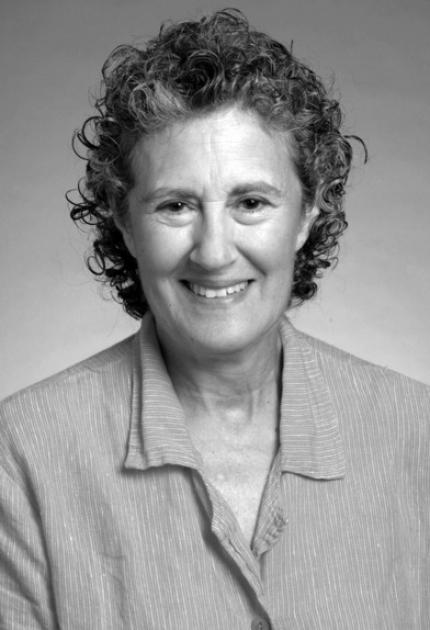
\includegraphics[scale=0.4, align=centre]{Barbara Liskov}
\centering

\end{frame}


%----------------------------------------------------------------------------------------
%	PRESENTATION SLIDES
%----------------------------------------------------------------------------------------

%------------------------------------------------


\begin{frame}
\frametitle{Title of page goes here}



\begin{itemize}
\end{itemize}
\end{frame}

%------------------------------------------------

\begin{frame}
\frametitle{Title of page goes here}

Writing here

\begin{itemize}
\item Bullet points go like this
\end{itemize}
\end{frame}

%------------------------------------------------

\begin{frame}
\frametitle{Title of page goes here}

1. Writing after number
\end{frame}

%------------------------------------------------
% NOTHING TO DO WITH LISKOV's PRINCIPLE,
% MATHS JUST HERE AS AN EXAMPLE
%-----------------------------------------------


\begin{frame}
\frametitle{Question 3: Steps of Finding Price Elasticity}
\begin{block}{Step 1: Obtain the Demand Curve After 1964}
$$ \left\{
\begin{aligned}
1500 = 562000a + b\\
1800 = 538000a + b\\
\end{aligned}
\right.\Rightarrow
P_{\textit{after}} = -\dfrac{1}{80} Q_{\textit{after}} + 8525
$$
\end{block}

\begin{block}{Step 2: Obtain the Demand Curve Before 1964}
$$ \left\{
\begin{aligned}
Q_{\pi_{max}} &= 40d\\
1350 &= -\dfrac{1}{80} 40d + d\\
\end{aligned}
\right.\Rightarrow
P_{\textit{before}} = -\dfrac{1}{80} Q_{\textit{before}} + 2700
$$
\end{block}

\begin{block}{Step 3: Obtain the Elasticity}
$$ \left\{
\begin{aligned}
P_{\textit{after}} &= -\dfrac{1}{80} Q_{\textit{after}} + 8525\\
P_{\textit{before}} &= -\dfrac{1}{80} Q_{\textit{before}} + 2700\\
\end{aligned}
\right.\Rightarrow
E_{(Q,P)}
$$
\end{block}
\end{frame}

%------------------------------------------------
% NOTHING TO DO WITH LISKOV's PRINCIPLE,
% MATHS JUST HERE AS AN EXAMPLE
%-----------------------------------------------

\begin{frame}
\frametitle{Title goes here}
\begin{theorem}[Title]
\centering
If the linear demand curve is unit elastic or $E_{(P,Q)}= -1$:\\
Then $MR = 0$
\end{theorem}
\end{frame}

%------------------------------------------------

\begin{frame}
\frametitle{Title}
\end{frame}

%------------------------------------------------


\begin{frame}
\frametitle{Title}
\end{frame}

%------------------------------------------------

\begin{frame}
\frametitle{Title}
\end{frame}

%------------------------------------------------

\begin{frame}
\Huge{\centerline{The End}}
\end{frame}

%----------------------------------------------------------------------------------------

\begin{frame}
\Huge{\centerline{Questions?}}
\end{frame}

%-----------------------------------------------
\end{document} 